While it has been stated that filters of smaller size are not suitable to recognize the complex relationships between Chinese strokes in convolutional architectures\cite{conv-chinese-character-synthesis}, this is overlooking fundamental hierarchies and geometric properties of logographic drawings.

Many approaches have focused on a specific language or script, for example Chinese\cite{online-ch}, Japanese\cite{online-ja}, or Korean\cite{offline-kr}. However, the structure can be generalized across CJK characters. In order to classify unseen characters, or a large number of characters, the intuition is that an approach leveraging these similarities be taken.

\subsection{Phono-semantic Compound Structure of Chinese characters}

Similar to the tree structure created by hyponyms and hypernyms of language which are captured within WordNet \cite{wordnet}, there exists a phono-semantic compound structure within many individual Chinese characters. Recent research on native Chinese speakers has shown the Stroop effect to occur, delaying recognition if misrepresented \cite{cjk-stroop}, indicating that the character recognition pathway within humans relies on these compounds. By decomposing compound ideographs into their constituent radicals, a graph can be created similar to the morphological decomposition and semantic field relationships within English. As over 80\% of the Chinese characters have been found to have this relationship \cite{compound-ideographs}. The intuition is that this structure is critical to obtaining fast character recall, creating a meaningful attention mechanism, and increasing performance in zero-shot classification.

\begin{figure}[h]
    \begin{center}
        \tikz[
        every shadow/.style={opacity=0.8,fill=blue!50!black},
        every pin/.style={font=\footnotesize}] {

            % Plant
            \node[shape=semicircle,shape border rotate=180, fill=cyan!20, inner sep=0.535cm] at (0, .95) {};
            \node[name=plant,circle split,very thick,pin=90:$semantic$,draw] at (0, 1.5) {\Huge 艹\nodepart{lower} plant};

            % Harvest
            \node[shape=semicircle,shape border rotate=180, fill=red!20, inner sep=0.575cm] at (0, -2.05) {};
            \node[name=harvest,set=component,circle split,very thick,pin=270:$phonetic$,draw] at (0, -1.5) {\Huge 采\nodepart{lower} harvest};

            % Claw
            \node[shape=semicircle,shape border rotate=180, fill=magenta!20, inner sep=0.535cm] at (-4.5, .95) {};
            \node[name=claw,circle split,very thick,draw] at (-4.5, 1.5) {\Huge ⺤\nodepart{lower} claw};

            % Tree
            \node[shape=semicircle,shape border rotate=180, fill=yellow!20, inner sep=0.575cm] at (-4.5, -2.05) {};
            \node[name=tree,circle split,very thick,draw] at (-4.5, -1.5) {\Huge 木\nodepart{lower} tree};

            % Vegetable
            \node[shape=semicircle,shape border rotate=180, fill=black!10, inner sep=0.575cm] at (4.5, -.575) {};
            \node[name=c,circle split,pin=90:$compound$,draw,very thick, double distance=2pt] at (4.5, 0) {\Huge 菜\nodepart{lower} vegetable};

            \begin{scope}[line width=2pt, arrows={-Stealth[length=10pt,inset=2pt]}]
               \draw (harvest) -> (c);
               \draw (plant) -> (c);
               \draw (claw) -> (harvest);
               \draw (tree) -> (harvest);
            \end{scope}
        }
        \caption[The Phono-semantic Relationship]{The phono-semantic relationship within the compound character, 菜 or \textit{vegetable}. The semantic component is a linguistic \textit{determinative}, providing the compound with elemental context. The phonetic component is semantically relevant here. Combined as \textit{"harvested plant"} for the character meaning \textit{vegetable}.}
        \label{fig:figure1}
    \end{center}
\end{figure}

\subsection{Kangxi Radical Position Encodings}

Kangxi radicals are the 214 radicals/roots comprising the compound characters of Chinese characters in CJK languages. As there are much fewer roots than possible constituents, positional encoding serves as a meta-feature necessary for classification beyond any base set.

In the Japanese encoding system, constituents are split into seven groups. These are \textit{top}, \textit{bottom}, \textit{left}, \textit{right}, \textit{kamae} (かまえ), \textit{tare} (たれ), and \textit{nyou} (にょう). The last three do not have equivalent words in English, but roughly translate to "enclosure", "hang down", and "wrap around bottom" respectively. The remaining case is for radicals themselves, which do not have a position. Totaling to a feature vector of size 8.

It is worth noting that the \textit{kamae} group represented by $\tikz\pic[color=gray, scale=0.6] at (0, -5pt) {kamae};$ in Figure \ref{fig:positions} is actually a grouping of positions that enclose another, but are less common than \textit{tare} or \textit{nyou}, and do not have a specific group. For example, 医 consists of \textit{kamae} radical 匚 enclosing 矢. The radical 匚 does not have an explicit stroke closing right side, although it can be thought of as being closed by deliberately missing stroke, differentiating it from 囗. Similarly, the radical 凵 is enclosed by a missing stroke on the top.

\begin{figure*}[t]
    \begin{center}
        \tikzset {
    shape kanjiframe/.style= {
        color=black!40,
        draw,
        fill=white,
        ultra thick,
    }
}

\def\defkanjipos#1#2 {
    \tikzset {
        #1/.pic = {
            \begin{scope}[every path/.style={color=black!40}]
            \pgftransformscale{0.5}
            \draw[rounded corners=1pt, shape kanjiframe] (0,0) rectangle (1,1);
            #2
            \end{scope}
            % \fill[fill=black!40] (0,0) rectangle ++(0.25, 0.5);
        }
    }
}

\defkanjipos{all}{
    \fill (0,0) rectangle (1,1);
}

\defkanjipos{top}{
    \fill (0,1) rectangle (1,0.5);
}

\defkanjipos{bottom}{
    \fill (0,0) rectangle (1,0.5);
}

\defkanjipos{left}{
    \fill (0,0) rectangle (0.5,1);
}

\defkanjipos{right}{
    \fill (0.5,0) rectangle (1,1);
}

\defkanjipos{kamae}{
    \fill (0,0) rectangle (1/3,1);
    \fill (2/3,0) rectangle ++(1/3,1);
    \fill (0,0) rectangle (1,1/3);
    \fill (0,2/3) rectangle ++(1,1/3);
}

\defkanjipos{tare}{
    \fill (0,0) rectangle (1/3,1);
    \fill (0,1) rectangle (1,2/3);
}

\defkanjipos{nyou}{
    \fill (0,0) rectangle (1/3,1);
    \fill (0,1/3) rectangle (1,0);
}

\defkanjipos{none}{}

\tikz {
    \foreach \x / \name in {0/top,1/bottom,2/left,3/right,4/kamae,5/tare,6/nyou,7/all} {
        \node at (0.25+\x,0.7) {\x};
        \pic at (\x,0) {\name};
    }
}

        \caption[Constituent Radical Positions]{The different positions of radicals within a CJK character. The encoded position uses 3 only bits. \newline From left to right: \(top\), \(bottom\), \(left\), \(right\), \(kamae\), \(tare\), \(nyou\), \(radical\)}
        \label{fig:positions}
    \end{center}
\end{figure*}

\subsection{Han Unification \& Unicode Ideographic Description Sequences}

To simplify similar character representations across Chinese (\textit{hanzi}), Japanese (\textit{kanji}), and Korean (\textit{hanja}) in the CJK languages, Unicode compresses similar representations into a single set of unified characters. This "Han unification" combines glyph variants by grapheme into a single code point within Unicode. The traditional Chinese glyph for "grass" uses four strokes in the radical (⺿), while simplified Chinese, Japanese, and Korean have three (⺾). The ⺿ and ⺾ characters both map to (U+8349, 草) and exist as variants. Due to the use as a radical, the four and three stroke variants contain separate encodings in the Unicode/CJK Radicals Supplement, allowing them to be rendered here.
Figure \ref{fig:han-unification} illustrates the effect on constituent radicals. The term \textit{ideograph} is used when referring to the set of glyph variants representing a common idea.

\begin{figure*}
    \begin{center}
        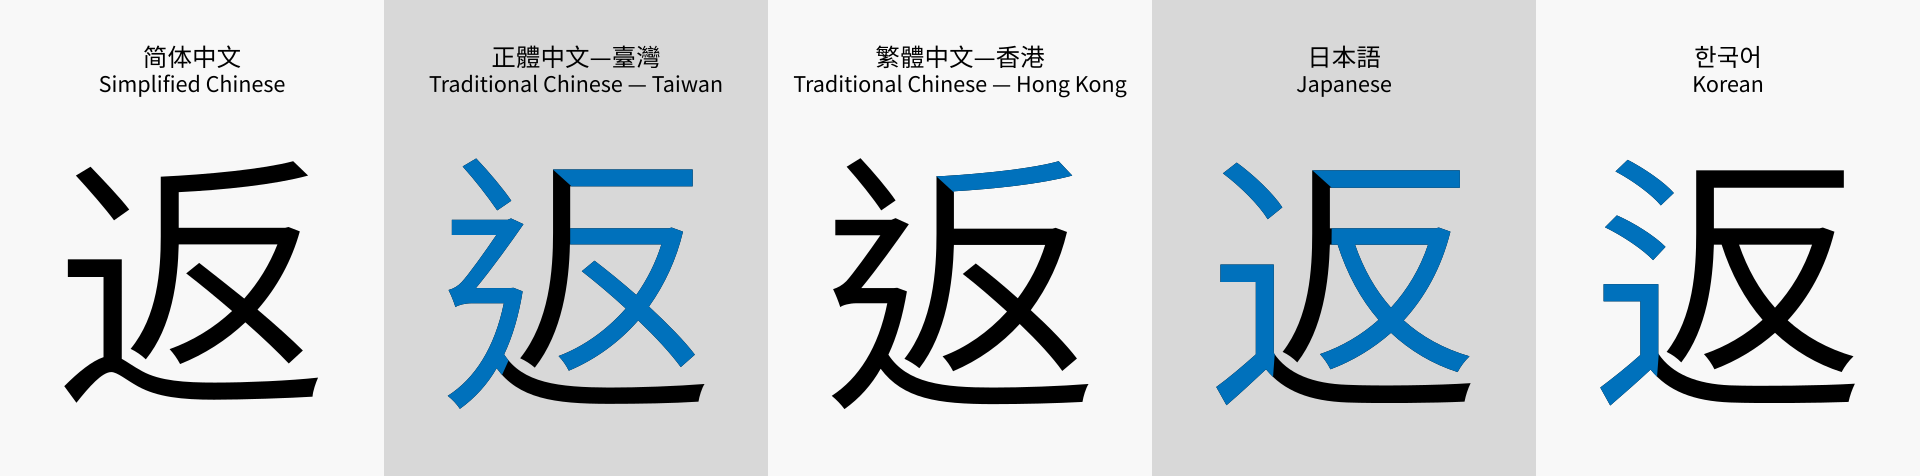
\includegraphics[width=1\textwidth]{figures/han_unification.png}
        \caption[Regional Character Variants]{Regional differences within the Unicode character (U+8FD4).
            Image in figure from Wikipedia\cite{wikipedia-han-unification}.}
        \label{fig:han-unification}
    \end{center}
\end{figure*}

Ideographic Description Sequences (IDS) in the Unicode standard\cite{unicode-ids} allows for any character to be encoded using logographic composition that is common across CJK characters. A representation sequence is shown in Figure \ref{fig:biang-ids}. Enocding sequences are not unique, and have a many-to-one relationship. The large quantity of strokes in the character \textit{biáng} in Figure \ref{fig:biang} illustrates that despite variations in constituents, a core set of ideographs determines the compound character meaning.

\begin{figure*}[h]
    \begin{center}
        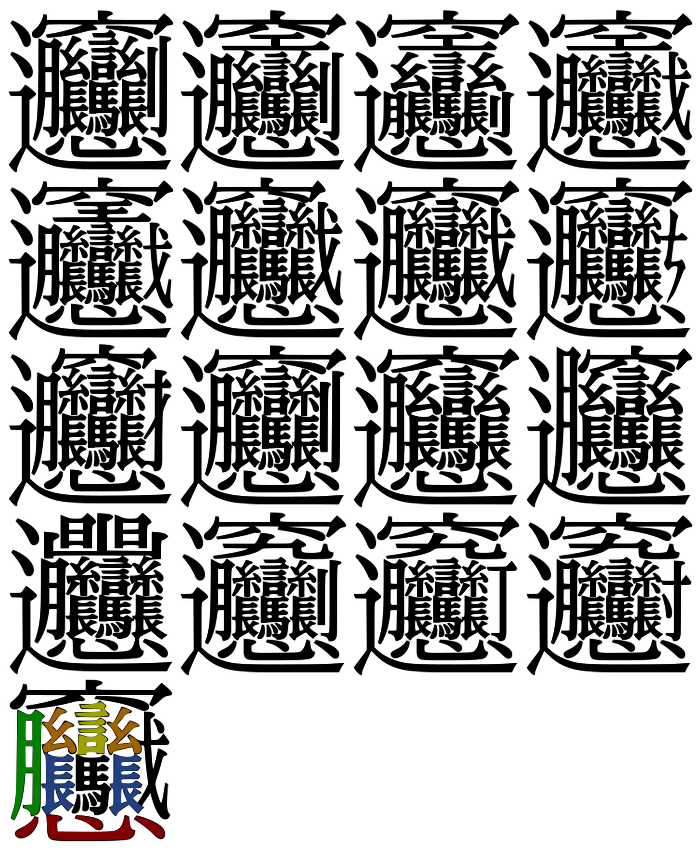
\includegraphics[width=0.3\textwidth]{figures/biang-variants.png}
        \caption[The 17 variants of \textit{biáng}]{The 17 variants of the character \textit{biáng}, a type of noodle. The last variant has constituents common across all variants colored to illustrate the core ideographs. \newline\textbf{These core constituents illustrate the intuition behind a bidirectional, multi-headed attention model.}}
        \label{fig:biang}
    \end{center}
\end{figure*}

\begin{figure*}[t]
    \begin{center}
        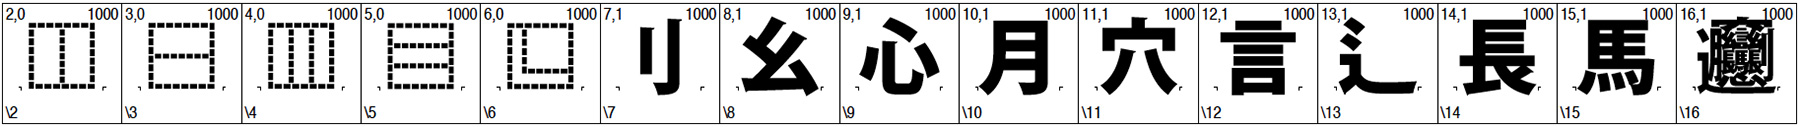
\includegraphics[width=1\textwidth]{figures/ids-biang.jpg}
        \caption[Unicode Ideographic Description Sequences]{An IDS of length 15 encoding the rendering of \textit{biáng} in OpenType. This sequence is just one capable of rendering \textit{biáng}, prior to it's inclusion in 2020\cite{unicode-ids}.
            Image in figure from Adobe \cite{adobe-ids}.}
        \label{fig:biang-ids}
    \end{center}
\end{figure*}
